\section{Multigrid Methods}
Multigrid methods have been designed to accelerate the convergence of iterative methods by eliminating certain error components on a so-called coarser representation of the original problem.
While the basic iterative methods discussed in the last section are applicable to many PDE-based problems, in practice, their speed of convergence is often insufficient, which means that a large number of iterations is required until an acceptable approximation accuracy can be attained. 
The main reason for this behavior is that these methods are only efficient in the reduction of certain error components, while others remain mostly unaffected~\cite{briggs2000multigrid}.
This can be best understood by considering the effect of a stationary iterative method on oscillatory errors of different frequency.
For this purpose, we consider the one-dimensional Laplace equation
\begin{equation}
		\begin{split}
			- \dv[2]{x} u(x) & = 0 \quad \forall x \in (0, 1) \\
			u(0) = u(1) & = 0,
		\end{split}
		\label{eq:1D-laplace-model}
\end{equation}
which is discretized using the three-point stencil
\begin{equation}
	\Delta_h^{(3, 1)} = \frac{1}{h^2}\begin{bmatrix}
		-1 & 2 & -1
	\end{bmatrix}.
		\label{eq:1D-laplace-stencil}
\end{equation} 
Figure~\ref{fig:different-error-components} shows the impact of applying the Jacobi´and Gauss-Seidel method on different periodic error components.
\begin{figure}
	\centering
	\begin{subfigure}[b]{0.32\textwidth}
		\centering
		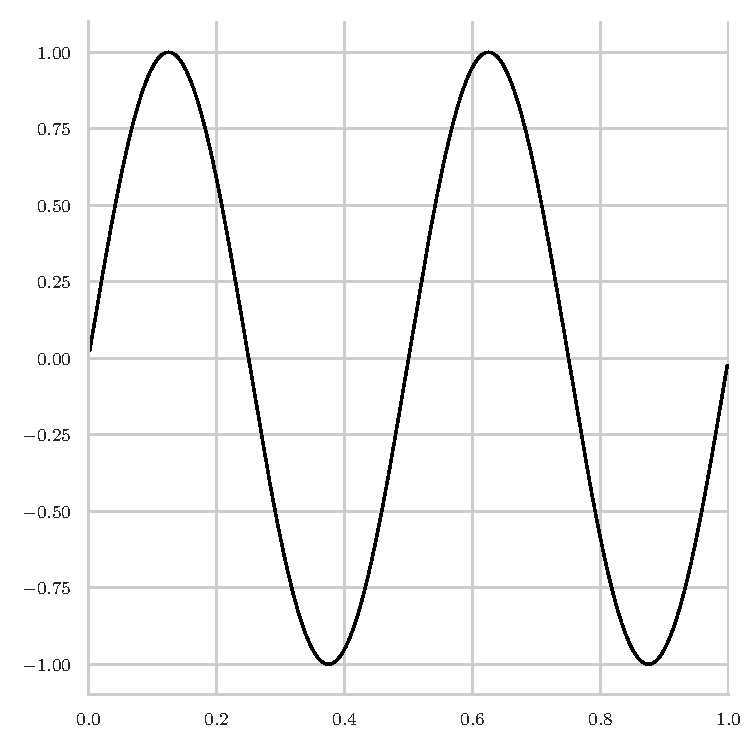
\includegraphics[width=\textwidth]{figures/initial_error_jacobi_4pi.pdf}
		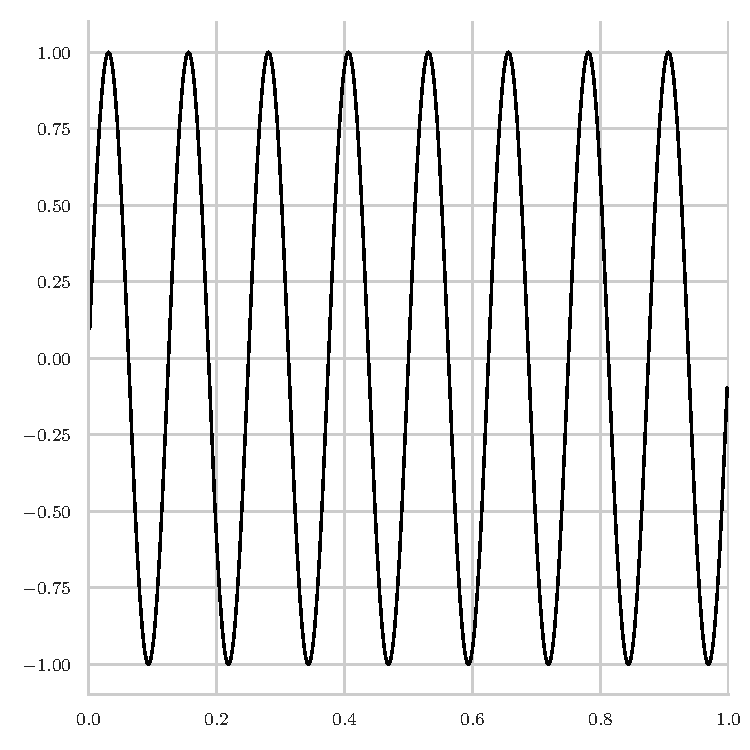
\includegraphics[width=\textwidth]{figures/initial_error_jacobi_16pi.pdf}
		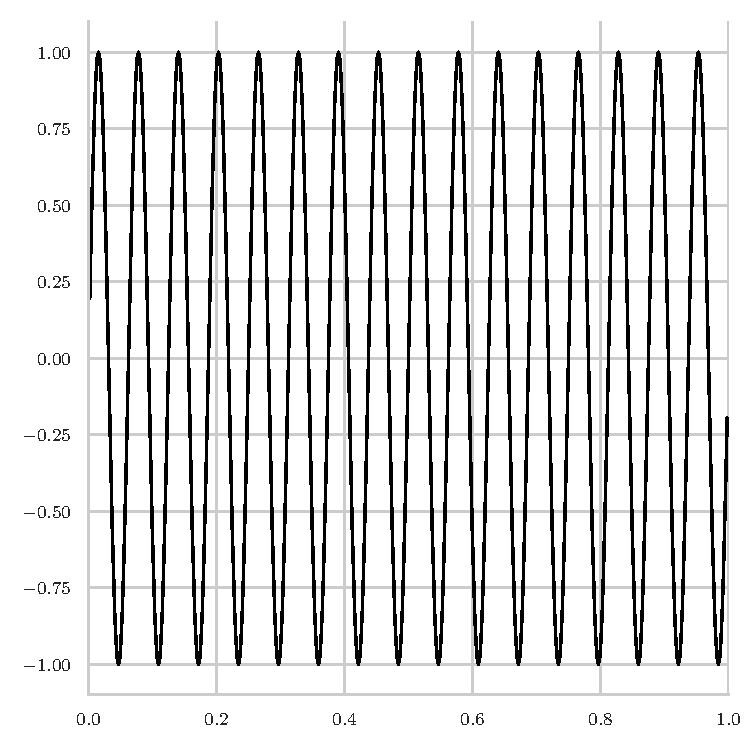
\includegraphics[width=\textwidth]{figures/initial_error_jacobi_32pi.pdf}
		\caption{Initial error}
	\end{subfigure}
	\hfill
	\begin{subfigure}[b]{0.32\textwidth}
		\centering
		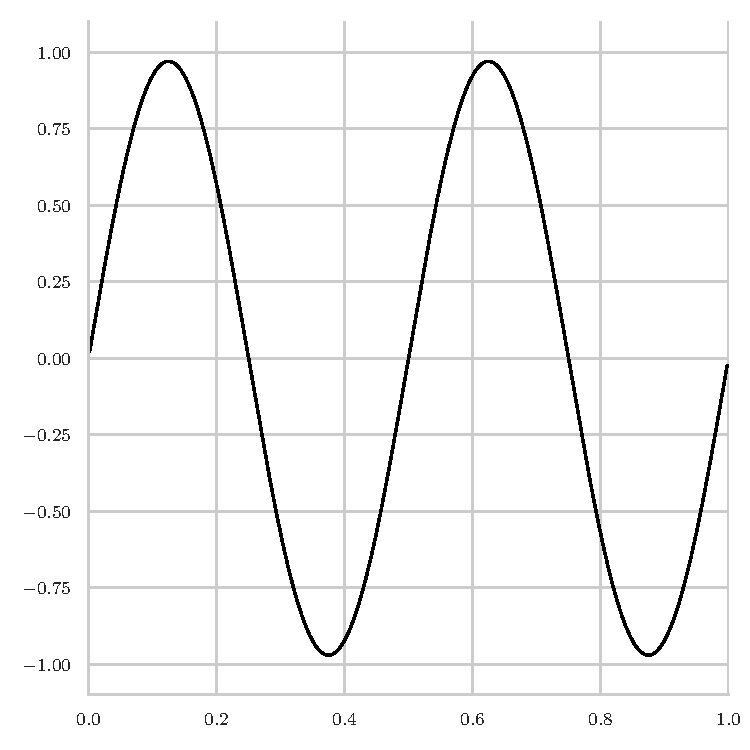
\includegraphics[width=\textwidth]{figures/final_error_jacobi_4pi.pdf}
		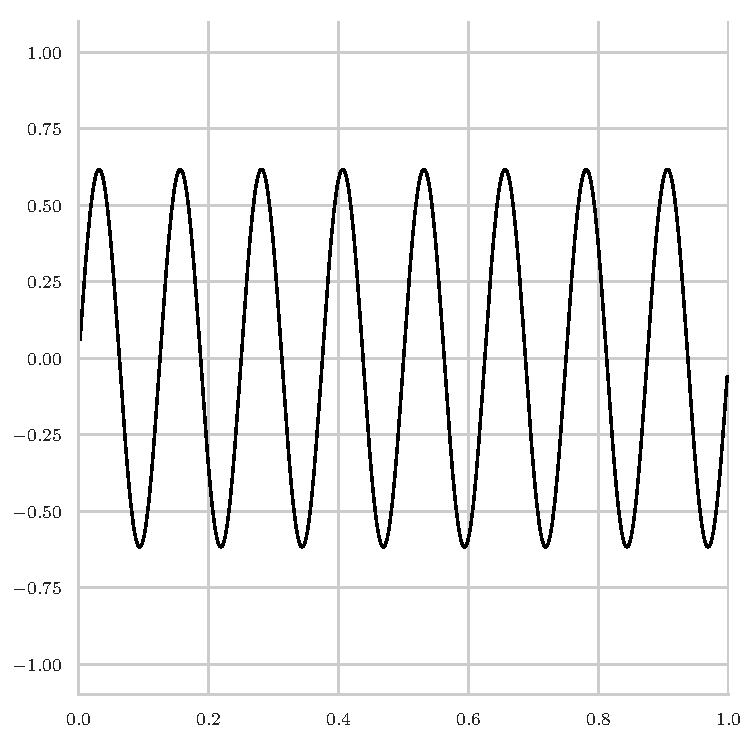
\includegraphics[width=\textwidth]{figures/final_error_jacobi_16pi.pdf}
		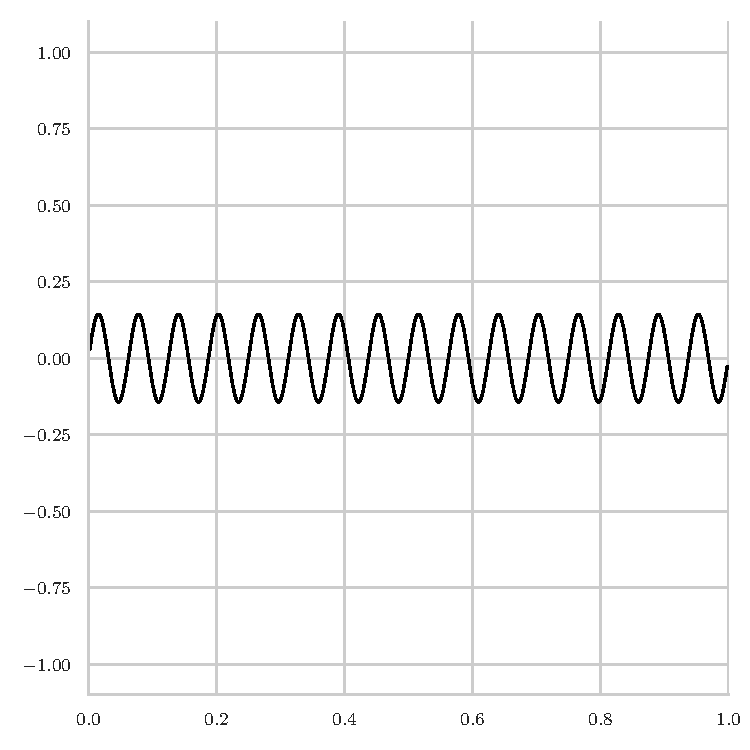
\includegraphics[width=\textwidth]{figures/final_error_jacobi_32pi.pdf}
	\caption{Error after applying Jacobi}
	\end{subfigure}
	\hfill
	\begin{subfigure}[b]{0.32\textwidth}
		\centering
		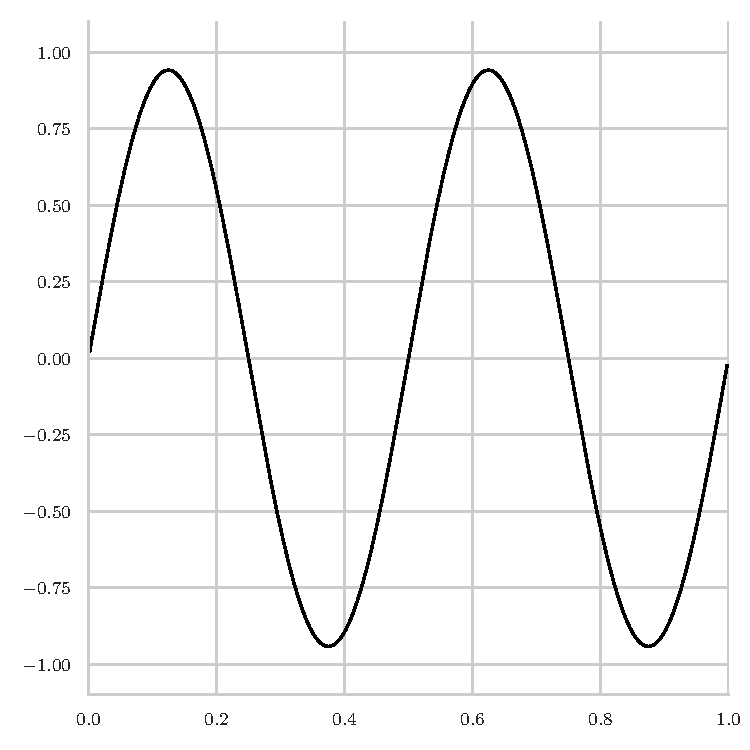
\includegraphics[width=\textwidth]{figures/final_error_gauss_seidel_4pi.pdf}
		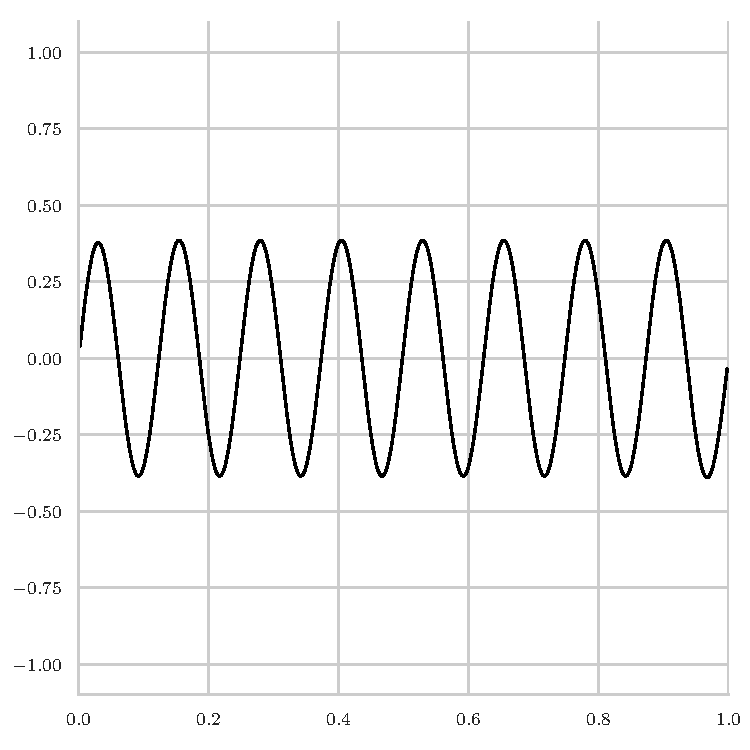
\includegraphics[width=\textwidth]{figures/final_error_gauss_seidel_16pi.pdf}
		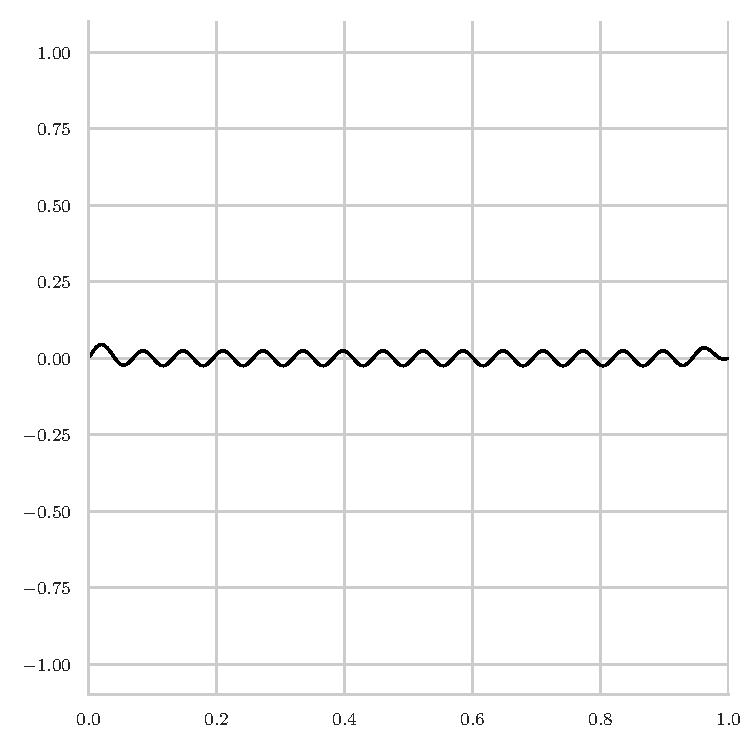
\includegraphics[width=\textwidth]{figures/final_error_gauss_seidel_32pi.pdf}
	\caption{Error after applying Gauss-Seidel}
	\end{subfigure}
	\caption{Different error components on a grid with step size $h = 2^{-9}$ before and after applying either 100 steps of the Jacobi or Gauss-Seidel method.}
	\label{fig:different-error-components}
\end{figure}
Here, the left column shows the initial error discretized on a grid with step size $h = 2^{-9}$ while the middle and right one includes the remaining error after applying 100 Jacobi and Gauss-Seidel steps, respectively.
Note that the frequency of change increases from top to bottom, whereas the amplitude of the error is always the same.
As it becomes apparent from investigating the middle and right columns of the first row of Figure~\ref{fig:different-error-components}, the Jacobi and Gauss-Seidel methods are both not able to achieve a significant reduction of those error components with a low frequency of change within 100 iterations.
In contrast, the third row, which represents a highly-oscillating component, the application of 100 steps of the Jacobi method already reduces the initial error to less than one-fifth of its original value.
The same behavior can also be observed for the Gauss-Seidel method, whereby, compared to the Jacobi method, high-frequency error components are reduced even faster.

We can further illustrate the error reduction properties of basic iterative methods by investigating Figure~\ref{fig:combined-error} which shows the combination of two error components with equal magnitude, one of them with low the other one with high frequency.
Again, the left plot shows the initial while the middle and right ones contain the reduced error after 100 iterations of Jacobi and Gauss-Seidel, respectively.
As it can be seen here, the attained improvement with both methods can be almost fully attributed to the reduction of the highly-oscillating component.
\begin{figure}
	\begin{subfigure}[b]{0.32\textwidth}
	\centering
		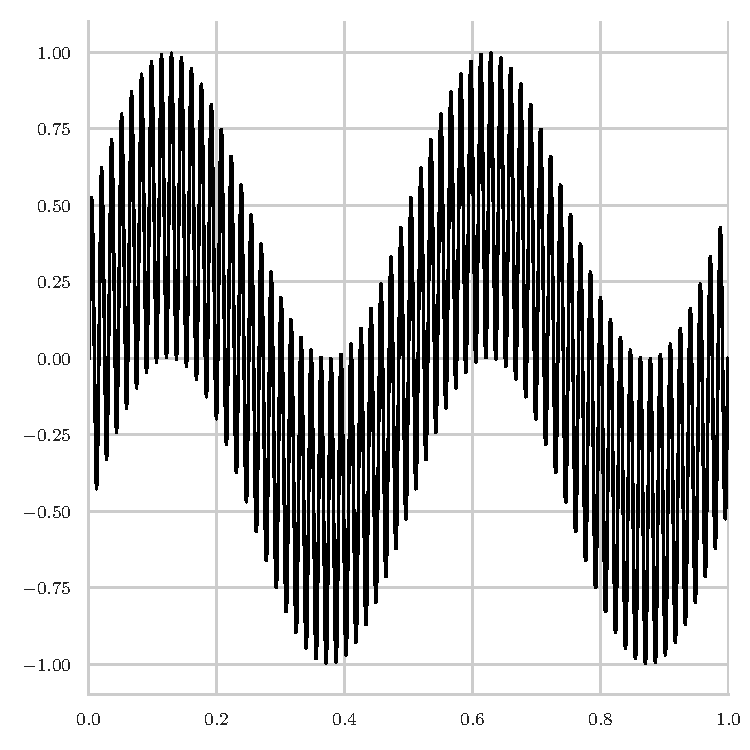
\includegraphics[width=\textwidth]{figures/initial_error_jacobi_combined.pdf}
		\caption{Initial error}
\end{subfigure}
\hfill
\begin{subfigure}[b]{0.32\textwidth}
	\centering
		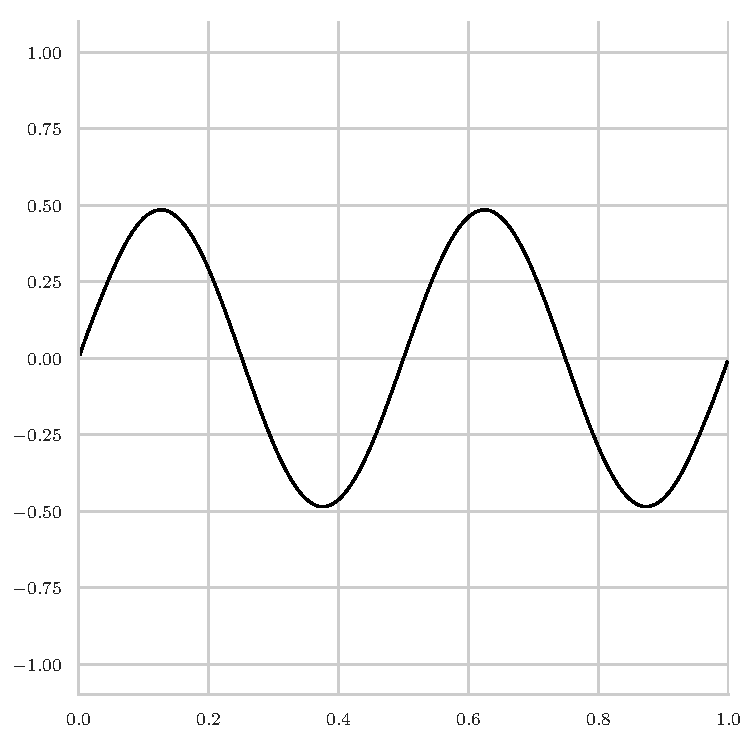
\includegraphics[width=\textwidth]{figures/final_error_jacobi_combined.pdf}
		\caption{Error after applying Jacobi}
\end{subfigure}
\begin{subfigure}[b]{0.32\textwidth}
	\centering
	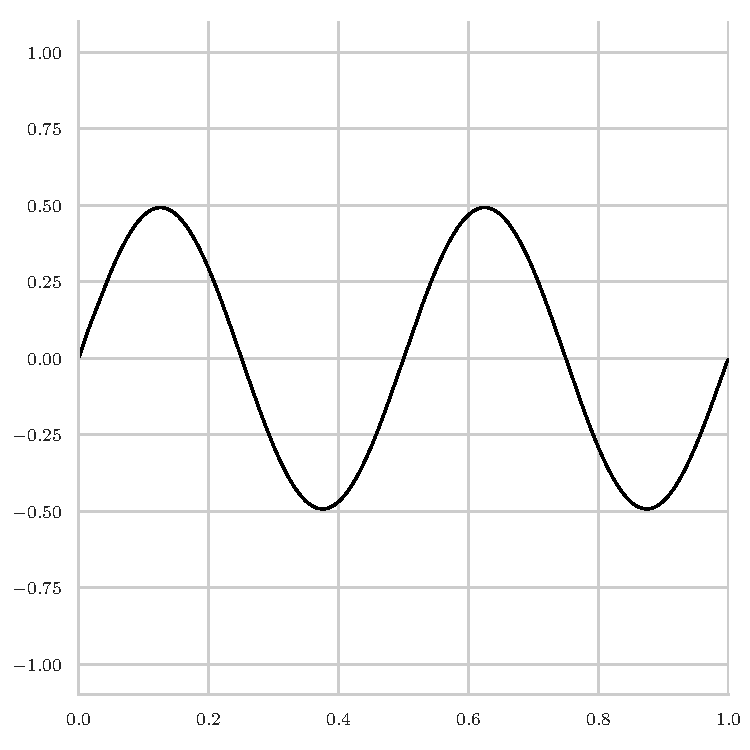
\includegraphics[width=\textwidth]{figures/final_error_gauss_seidel_combined.pdf}
	\caption{Error after applying Gauss-Seidel}
\end{subfigure}
	\caption{Combination of two error components discretized on a grid with step size $h = 2^{-9}$ before and after applying 100 steps of either the Jacobi or Gauss-Seidel method.}
\label{fig:combined-error}
\end{figure}
Because the remaining error is more smooth than initially, basic iterative methods are often denoted as \emph{smoothers} and their effectiveness is measured in terms of their capability to reduce the high-frequency components of a given error. 

Now observe what happens if we represent the same low-frequency error component shown in the first row of Figure~\ref{fig:different-error-components} on a grid with larger step size $h = 2^{-6}$, hence a smaller number of grid points.
Because the number of (inner) grid points $n$ is inversely proportional to the step size with $n = 1/h - 1$, usually the term \emph{coarser} grid is used.
The resulting error reduction, again after 100 iterations of each of both iterative methods, is shown in Figure~\ref{fig:low-frequency-error-component-coarse}. 
\begin{figure}
	\begin{subfigure}[b]{0.32\textwidth}
	\centering
	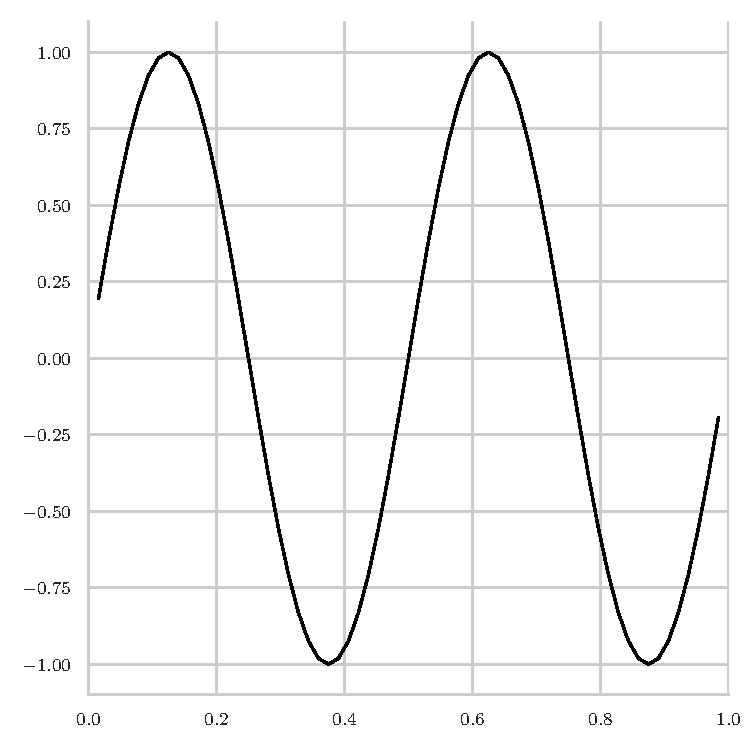
\includegraphics[width=\textwidth]{figures/initial_error_jacobi_4pi_coarse.pdf}
	\caption{Initial error}
\end{subfigure}
\hfill
\begin{subfigure}[b]{0.32\textwidth}
	\centering
	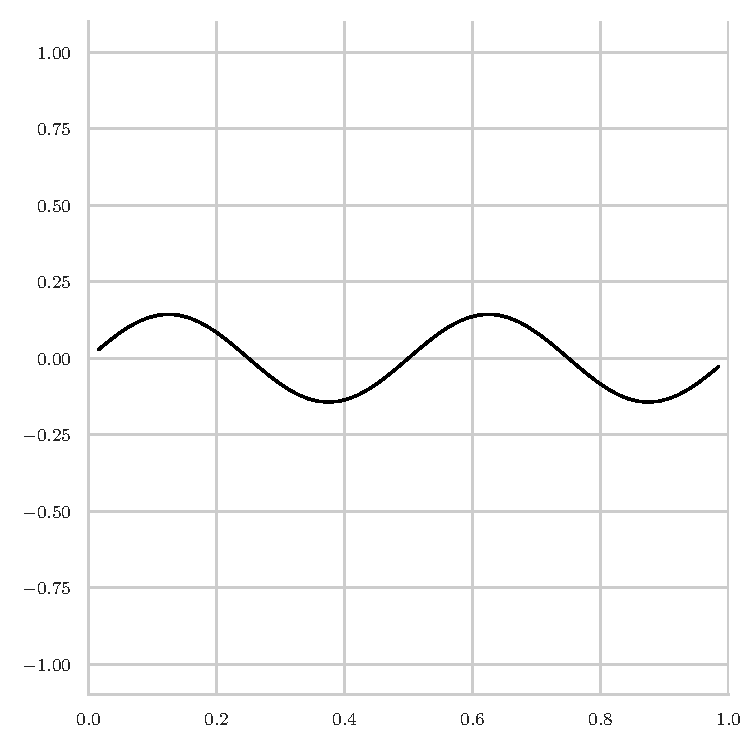
\includegraphics[width=\textwidth]{figures/final_error_jacobi_4pi_coarse.pdf}
	\caption{Error after applying Jacobi}
\end{subfigure}
	\hfill
	\begin{subfigure}[b]{0.32\textwidth}
		\centering
		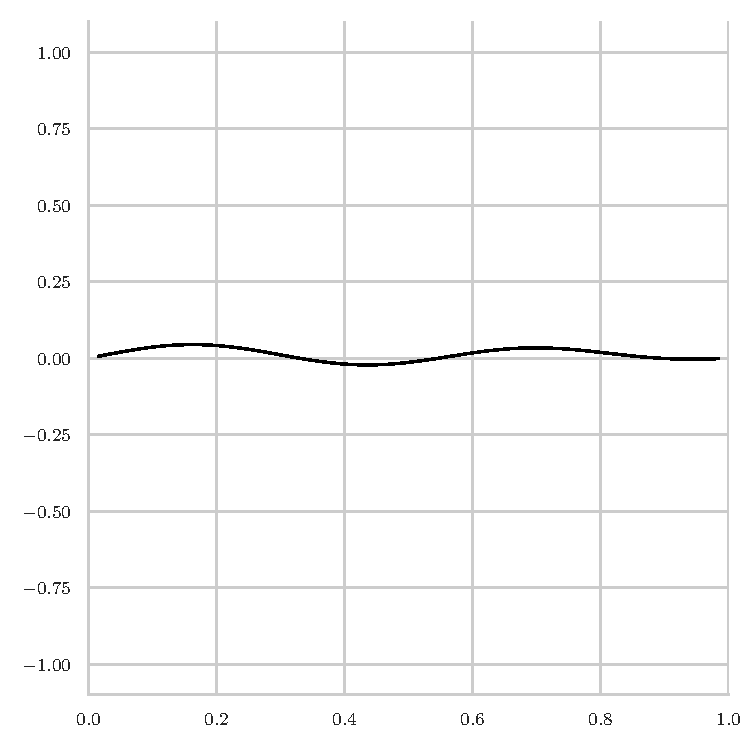
\includegraphics[width=\textwidth]{figures/final_error_gauss_seidel_4pi_coarse.pdf}
		\caption{Error after applying Gauss-Seidel}
	\end{subfigure}
	\caption{Low-frequency error component discretized on a coarse grid with step size $h = 2^{-6}$ before and after applying 100 steps of either the Jacobi or Gauss-Seidel method.}
	\label{fig:low-frequency-error-component-coarse}
\end{figure}
As it can be seen, the amount of low-frequency error reduction is significantly higher for both methods than on the \emph{finer} grid with a step size of $h = 2^{-9}$.
While basic iterative methods, like the Jacobi and Gauss-Seidel method are only capable of reducing the high-frequency components of a given error, we can, hence, employ the same methods to effectively reduce the remaining low-frequency components when they can be represented on a coarser grid.
\emph{Multigrid} methods build up on this idea by automating the process of recursively obtaining a coarser representation of a given problem, which can then be effectively reduced by employing only a few \emph{smoothing} iterations.
These methods, therefore, operate on a so-called hierarchy of grids, where on each subsequent discretization level certain error components are reduced, which is then used to correct the remaining error on the next-finer grid.
In the following, we first introduce the basic components of a multigrid method, such as the smoothing, restriction, prolongation and coarse grid correction operations.
Based on this definition, we then develop a formal language for the representation of multigrid solvers.
\subsection{Smoothing}
\label{subsec:smoothing}
One of the central elements of multigrid methods is the utilization of a smoothing procedure, that is able to quickly reduce the oscillatory components of a given error.
We have already shown that the Jacobi and Gauss-Seidel method behave in such a way for the considered one-dimensional model problem.
To further improve the smoothing property of a basic iterative methods, it is often beneficial to introduce an additional relaxation factor $\omega$ which yields the iteration 
\begin{equation}
	\bm{x}^{(i+1)} = \bm{x}^{(i)} + \omega M^{-1}(\bm b - A \bm{x}^{(i)}).
	\label{eq:general-weighted-stationary-iterative-method}
\end{equation}
Again, a weighted Jacobi or Gauss-Seidel can then be obtained by replacing the matrix $M$ by the respective term.
\subsubsection{Red-Black Gauss-Seidel}
While the Gauss-Seidel method exhibits superior smoothing properties compared to the Jacobi method, each iteration requires solving a lower triangular system of the form
\begin{equation*}
	(D - L) (\bm{x}^{(k+1)} - \bm{x}^{(k)}) = \bm{b} - A \bm{x}^{(k)},
\end{equation*}
with $D - L$ as the lower triangular part of the system matrix $A$.
Since $U = A - (D - L)$, we can rewrite this equation to obtain
\begin{equation*}
	(D - L) \bm{x}^{(k+1)} = \bm{b} - U \bm{x}^{(k)}.
\end{equation*}  
which can then be solved using forward substitution by applying
\begin{equation}
	x_{i}^{(k+1)}={\frac {1}{a_{ii}}}\left(b_{i}-\sum _{j=1}^{i-1}a_{ij}x_{j}^{(k+1)}-\sum _{j=i+1}^{n}a_{ij}x_{j}^{(k)}\right),
	\label{eq:gauss-seidel-element-wise}
\end{equation}
where $x_{i}^{(k)}$ represents the $i$th element of the vector $\bm{x}^{(k)}$.
However, because $x_{i+1}^{(k)}$ depends on $x_{i}^{(k)}$ this computation can must be performed sequentially, which means that the individual components of $\bm{x}^{(k+1)}$ must be computed one after another. 
Modern compute architectures exhibit an ever increasing degree of parallelism and, therefore, rely on the fact that all computations can be performed fully in parallel.
For comparison, consider the Jacobi method as defined by 
\begin{equation*}
	\bm{x}^{(k+1)} = \bm{x}^{(k)} + D^{-1}(\bm b - A \bm{x}^{(k)}).
\end{equation*}
Similar to the Gauss-Seidel method, we can first rewrite this equation to
\begin{equation*}
	\bm{x}^{(k+1)} = D^{-1}(\bm b - (A - D)\bm{x}^{(k)}),
\end{equation*}
which then yields the following element-wise formulation of the Jacobi method:
\begin{equation}
x_{i}^{(k+1)}={\frac {1}{a_{ii}}}\left(b_{i}-\sum _{j\neq i}a_{ij}x_{j}^{(k)}\right).
	\label{eq:jacobi-element-wise}
\end{equation}
In contrast to Equation~\eqref{eq:gauss-seidel-element-wise} the computation of each subsequent element of the vector $\bm{x}^{(k+1)}$ does not depend on any of its previous ones.
Consequently, the computation of a new approximate solution $\bm{x}^{(k+1)}$ using the Jacobi method can be performed in parallel for each individual element of the vector.

One possibility to enable a parallel computation of the approximate solution $\bm{x}^{(k+1)}$ that is similar to the Gauss-Seidel method but does not rely on a sequential computation, is to partition the grid points into multiple subsets.
The computation of each subset is then performed in a Jacobi-like fashion, however, in case the values of grid points from other subsets are needed, the updated values are used.
A common variant of this approach is the red-black Gauss-Seidel method.
Here, the grid points are assigned to two distinct sets, where the first represents the red and the second one the black points.
We can define the red-black Gauss-Seidel method in the following way:
\begin{equation}
	\begin{split}
		\bm{x}^{(k+1/2)} & = \bm{x}^{(k)} + P_r D^{-1} (\bm{b} - A \bm{x}^{k}) \\
		\bm{x}^{(k+1)} & = \bm{x}^{(k+1/2)} + P_b D^{-1} (\bm{b} - A \bm{x}^{k+1/2})
	\end{split}
\end{equation}
The entries of the matrices $P_R$ and $P_B$ are then defined as
\begin{equation}
	P_{R,ij} = \begin{cases}
	1 & \text{if} \; i = j \; \text{and} \; i,j \in R \\
	0 & \text{otherwise},  
	\end{cases}
\end{equation}
\begin{equation}
	P_{B,ij} = \begin{cases}
		1 & \text{if} \; i = j \; \text{and} \; i,j \in B \\
		0 & \text{otherwise}  
	\end{cases}
\end{equation}
Here, $R$ and $B$ are the sets of grid indices that correspond to the red and black points, respectively.
Now consider again the three-point stencil defined in Equation~\eqref{eq:1D-laplace-stencil}.
If we define the Gauss-Seidel method with respect to this stencil we obtain
\begin{equation*}
	x_{i}^{(k+1)}=\frac {1}{2}\left(b_{i} + x_{i-1}^{(k+1)} + x_{i+1}^{(k)}\right).
\end{equation*}
Here the update of each individual grid point is exclusively based on its neighbors, whereas the left neighbor $x_{i-1}^{(k+1)}$ has already been updated in the previous step of the method.
We can achieve a similar behavior by assigning neighboring grid points to different partitions, for instance in case of a red-black partitioning by defining
\begin{equation}
		R = \{ \bm{i} : \bm{i} \in \mathbb{N}^d, \sum_{k=1}^d i_k \; \text{even} \}, \;
		B = \{ \bm{i} : \bm{i} \in \mathbb{N}^d, \sum_{k=1}^d i_k \; \text{odd} \}.
\end{equation}
In many cases, the resulting method has better smoothing properties than the Jacobi method without sacrificing much of its parallelism, since the computations on each partition can be performed in parallel~\cite{trottenberg2000multigrid}.
\subsubsection{Block Smoothing}
In Section~\ref{subsec:smoothing}, we have only discussed smoothers that operate in a pointwise manner.
For instance, in the Jacobi method, Equation~\eqref{eq:jacobi-element-wise} is computed for each individual grid point.
The idea of block smoothing is to reorder the original system in such a way, that the same operations can be defined on blocks of grid points.
As a consequence each scalar operation in the original pointwise method is then replaced by a matrix or vector operation, whose dimensionality corresponds to the chosen block size.

For example, we can rearrange our original system of the form of Equation~\eqref{eq:general-system-of-linear-equations} in the following way:
\begin{equation}
\underbrace{
\begin{pmatrix}A_{11}&A_{12}&\cdots &A_{1m}\\A_{21}&A_{22}&\cdots &A_{2m}\\\vdots &\vdots &\ddots &\vdots \\A_{m1}&A_{m2}&\cdots &A_{mm}\end{pmatrix}}_{A}
 = 
\underbrace{
\begin{pmatrix}
\bm{x}_1 \\ \bm{x}_2 \\ \vdots \\ \bm{x_m} 
\end{pmatrix}}_{\bm{x}} =
\underbrace{
\begin{pmatrix}
	\bm{b}_1 \\ \bm{b}_2 \\ \vdots \\ \bm{b_m} 
\end{pmatrix}}_{\bm{b}}
\end{equation}
with $m = n / n_b$ if $n_b$ is the size of each block.
A block Jacobi method can then be defined as
\begin{equation}
	\bm{x}_{i}^{(k+1)}=A_{ii}^{-1}\left(\bm{b}_{i}-\sum _{j\neq i}A_{ij}\bm{x}_{j}^{(k)}\right),
	\label{eq:jacobi-block-wise}
\end{equation}
For example we can define a block consisting of two elements for the one-dimensional Laplace equation and obtain the respective block Jacobi for each inner block with index $i$ by computing
\begin{equation}
	\begin{pmatrix}
		2 & -1 \\
		-1 & 2
	\end{pmatrix}
	\begin{pmatrix}
		x_{j}^{(k+1)} \\ x_{j+1}^{(k+1)} 
	\end{pmatrix}
= 	-  \begin{pmatrix}
	0 & 0 \\
	-1 & 0
\end{pmatrix} 	
\begin{pmatrix}
x_{j+2}^{(k)} \\ x_{j+3}^{(k)}
\end{pmatrix} -
\begin{pmatrix}
	0 & -1 \\
	0 & 0
\end{pmatrix} 	
\begin{pmatrix}
	x_{j-2}^{(k)} \\ x_{j-1}^{(k)} 
\end{pmatrix},
\end{equation}
where $j = n_b (i - 1) + 1$.
This method can be defined in a similar way using our previously introduced stencil notation
\begin{equation}
	\begin{pmatrix}
		\{(0, 2), (1, -1)\} \bullet x_{j}^{(k+1)} \\ \{(-1, -1), (0, 2)\} \bullet x_{j+1}^{(k+1)} 
	\end{pmatrix}
	= 	-
	\begin{pmatrix}
		\emptyset \bullet x_{j+2}^{(k)} \\ \{(-1, -1)\} \bullet x_{j + 3}^{(k)}
	\end{pmatrix} -
	\begin{pmatrix}
		\{(1,-1)\} \bullet x_{j-2}^{(k)} \\ \emptyset \bullet x_{j-1}^{(k)} 
	\end{pmatrix}.
\end{equation}
In both cases we obtain a system of two linear equation of the form
\begin{equation}
	\begin{pmatrix}
		2 x_{j}^{(k+1)} - x_{j+1}^{(k+1)} \\ 2 x_{j+1}^{(k+1)} - x_{j}^{(k+1)} 
	\end{pmatrix}
	=
	\begin{pmatrix}
		x_{j - 1}^{(k)} \\ x_{j + 2}^{(k)}
	\end{pmatrix}.
\end{equation}
that in each step of the method must be solved for each block, for instance, using a direct solver such as Gaussian elimination.
As in the pointwise Jacobi method, the system of each block can be solved independently and, therefore, operations on different blocks can be performed in parallel. 
Considering the fact that direct solvers in general require $\mathcal{O}(n_b^3)$ operations to solve each block, the overall computational cost of applying a block smoother can be estimated with $\mathcal{O}(n_b^3 \frac{n}{n_b}) = \mathcal{O}(n_b^2 n)$.
Note that choosing $n_b = n$ means that we treat the whole matrix $A$ as a single block and, therefore, solve the original system using Gaussian elimination.
In contrast, the choice of $n_b = 1$ corresponds to the pointwise Jacobi method, which, for a constant stencil, can be computed with a constant number of operations per grid point.
While we here only provide a brief introductions to block smoothers, it must be mentioned that it is also possible to define block variants for other smoothers, such as the Gauss-Seidel and red-black Gauss-Seidel method.
Finally, one can also define overlapping block smoothers needs, which means that multiple blocks contain the same grid point as an unknown to be solved.

\section{The coarse grid correction scheme}
The core idea behind multigrid methods is to reduce the oscillatory components of an error by obtaining an approximation of the same problem on a coarser grid.
As we have illustrated in Figure~\ref{fig:low-frequency-error-component-coarse} these components can then be reduced quickly using similar relaxation techniques that are effective to reduce oscillatory components on the finer grid.
Before defining this procedure, observe that our original system
\begin{equation}
	A \bm x = \bm b
\end{equation}
is equivalent to the error equation
\begin{equation}
	A \left(\bm{x} - \bm {x}^{(0)}\right) = \bm{b} - A \bm{x}^{(0)}
\end{equation}
with an arbitrary initial guess $\bm{x}^{(0)}$.
We can further introduce the error $\bm{e} = \bm{x} - \bm {x}^{(0)}$ to obtain the equation
\begin{equation}
	A \bm{e} = \bm{b} - A \bm{x}^{(0)}.
	\label{eq:linear-system-error-equation}
\end{equation}
The solution $\bm{e}$ of this system, which depends on the initial solution $\bm{x}^{(0)}$, can then be employed to obtain the solution of the original system by computing
\begin{equation}
	\bm{x} = \bm{x}^{(0)} + \bm{e}.
\end{equation}
Consequently, each approximate solution computed for Equation~\eqref{eq:linear-system-error-equation} can be used to obtain an approximation for the solution of the original system of linear equations.
Before we can define operations on a hierarchy of discretizations, we need to introduce the following notation:
The subscript $h$ indicates that an operator $A_h$ or the solution $\bm{x}_h$ is discretized on a (uniform) grid with step size $h$.  
Now, assume there exist the prolongation and restriction operators, $I_h^{2h}$ and $I_{2h}^h$, that enable us to obtain an approximation for a given variable $\bm{x}_h$ on a coarser and finer grid, respectively, such that
\begin{equation}
	\bm{x}_{2h} \approx I_h^{2h} \bm{x}_{h}, \;
	\bm{x}_{h} \approx I_{2h}^{h} \bm{x}_{2h}. 
\end{equation}
In general, this approximation can obviously never be exact.
However, we have already observed that a certain error only consists of smooth components, we can approximate the same components on a coarser grid without a significant loss of accuracy.
This is illustrated in Figure~\ref{fig:error-on-multiple-levels}, where two error components with different frequency are discretized on a hierarchy of grids with decreasing steps size.
Here, the first error component, which possesses a higher frequency, can not be accurately represented on the coarsest grid with step size $h = 2^{-5}$.
In contrast, the characteristics of the second error component, which is relatively smooth, is still clearly visible on the same grid. 
\begin{figure}
	\begin{subfigure}[b]{0.32\textwidth}
		\centering
		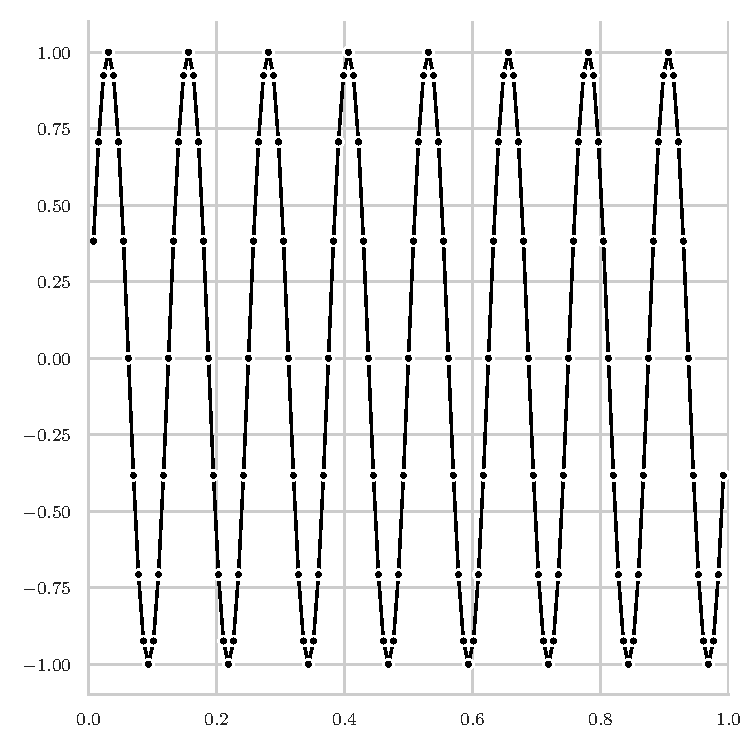
\includegraphics[width=\textwidth]{figures/initial_error_16pi_level7.pdf}
	\end{subfigure}
	\hfill
	\begin{subfigure}[b]{0.32\textwidth}
		\centering
		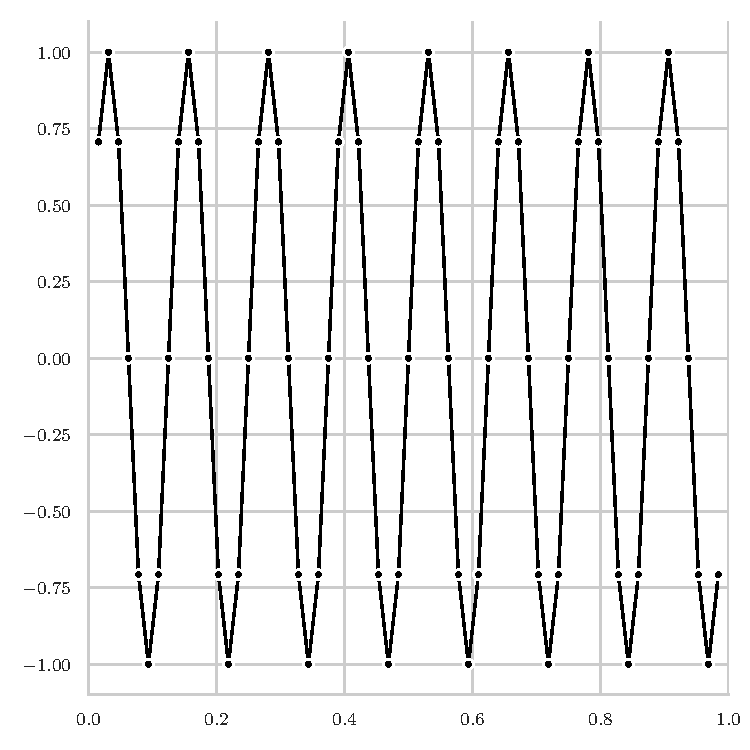
\includegraphics[width=\textwidth]{figures/initial_error_16pi_level6.pdf}
	\end{subfigure}
	\hfill
	\begin{subfigure}[b]{0.32\textwidth}
		\centering
		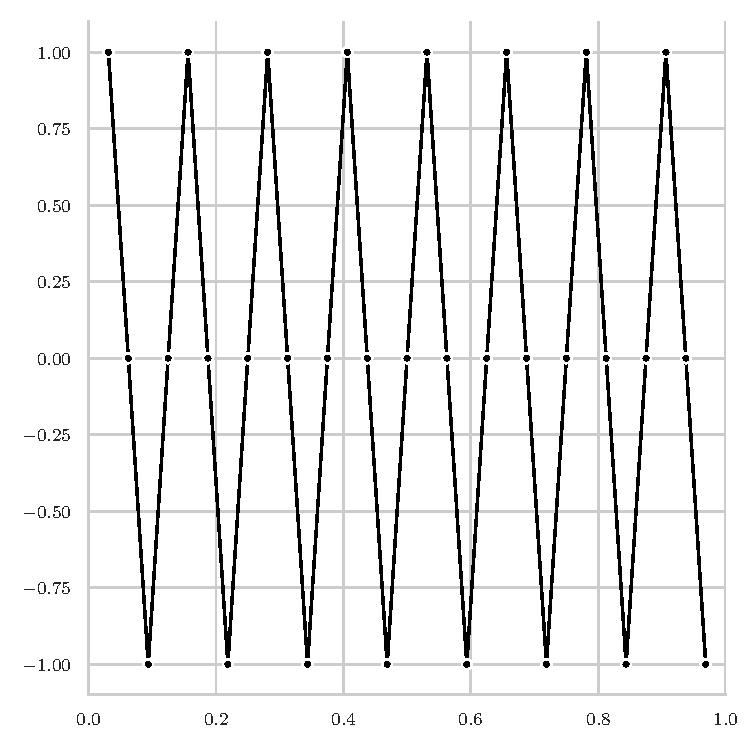
\includegraphics[width=\textwidth]{figures/initial_error_16pi_level5.pdf}
	\end{subfigure}
		\begin{subfigure}[b]{0.32\textwidth}
		\centering
		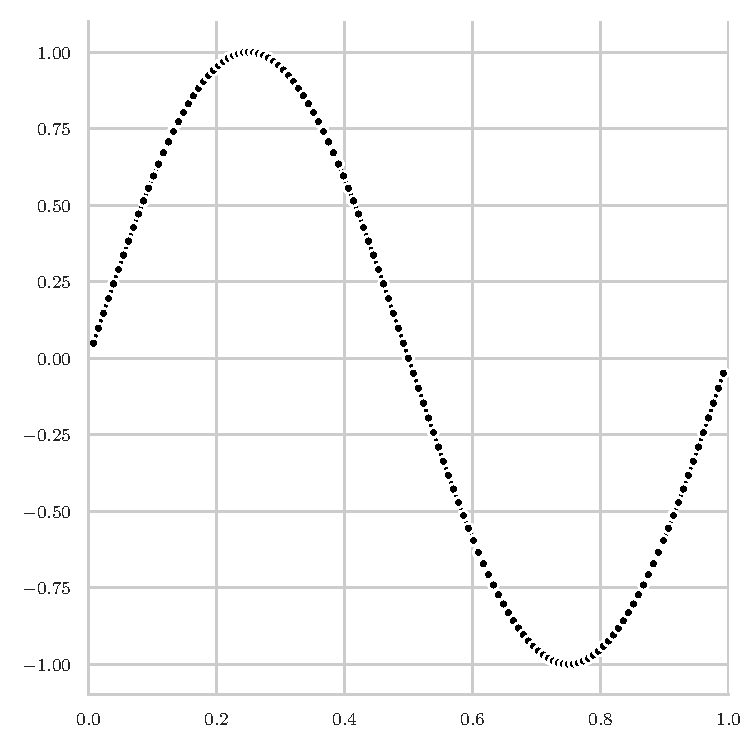
\includegraphics[width=\textwidth]{figures/initial_error_2pi_level7.pdf}
		\caption{$h = 2^{-7}$}
	\end{subfigure}
	\hfill
	\begin{subfigure}[b]{0.32\textwidth}
		\centering
		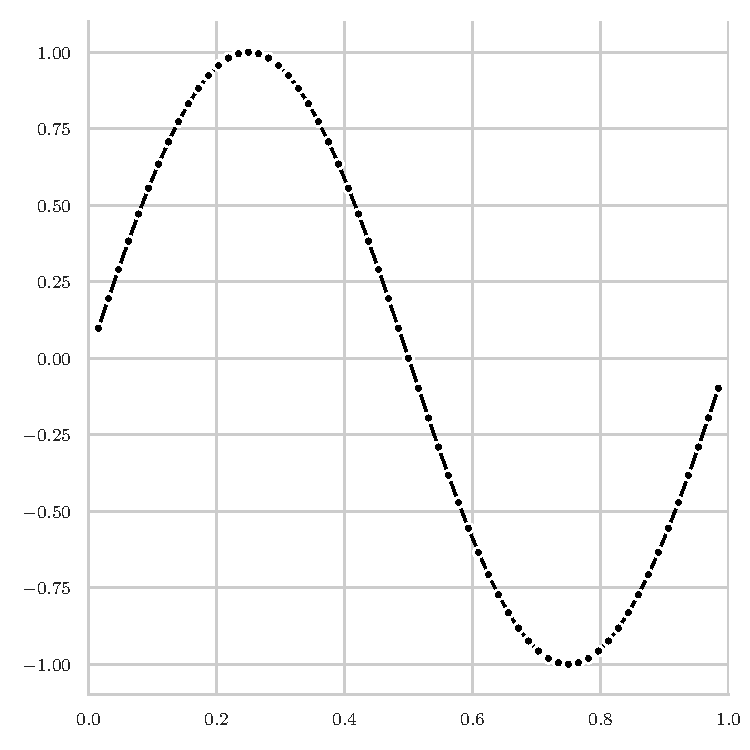
\includegraphics[width=\textwidth]{figures/initial_error_2pi_level6.pdf}
		\caption{$h = 2^{-6}$}
	\end{subfigure}
	\hfill
	\begin{subfigure}[b]{0.32\textwidth}
		\centering
		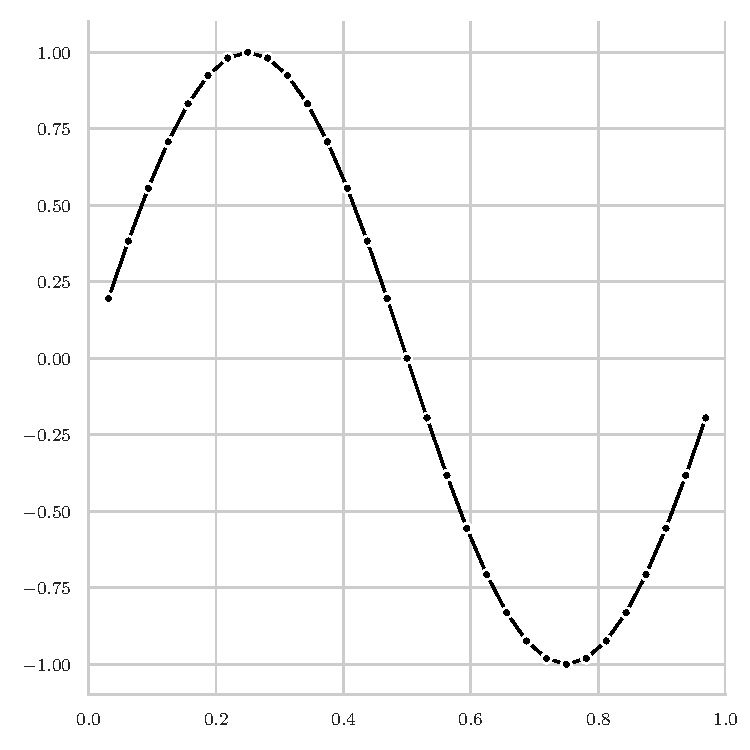
\includegraphics[width=\textwidth]{figures/initial_error_2pi_level5.pdf}
		\caption{$h = 2^{-5}$}
	\end{subfigure}
	\caption{Oscillatory and smooth error components discretized on a hierarchy of grids with decreasing step size.}
	\label{fig:error-on-multiple-levels}
\end{figure}
Assuming that the error $\bm{e}_{2h}$ on the coarse grid consists exclusively of smooth components and, hence, $\bm{e}_{h} \approx I_{2h}^{h} \bm{e}_{2h}$, we can define the coarse grid correction 
\begin{equation}
	\bm{x}^{k+1}_h = \bm{x}^{k}_h + I_{2h}^h \bm{e}_{2h}.
\end{equation} 
Now the question remains to be answered how we can compute the error $\bm{e}_{2h}$ on the coarse grid.
As we have shown Equation~\eqref{eq:linear-system-error-equation} is equivalent to the original system.
Therefore, we can apply our previously defined inter-grid transfer operators to define the coarse error equation
\begin{equation}
	\underbrace{I_{h}^{2h} A_h I_{2h}^h}_{A_{2h}} \bm{e}_{2h} = I_{h}^{2h} \left(\bm{b}_h - A \bm{x}^{(0)}_h\right).
	\label{eq:coarse-grid-error-equation}
\end{equation}
Note that we have again made use of the fact that $\bm{e}_{h} \approx I_{2h}^{h} \bm{e}_{2h}$ is a reasonably accurate approximation in case $\bm{e}_{2h}$ is smooth.
Note that in Equation~\eqref{eq:coarse-grid-error-equation} the coarse operator $A_{2h}$ is directly obtained from the original operator $A_{2h}$. 
This process is usually called \emph{Galerkin coarsening}.
However, in cases where the operator $A_h$ can be directly discretized on a coarser grid with step size $2h$, it is often also possible to use the resulting operator $A_{2h}$ instead.
%\subsection{Systems of PDEs}
%TODO write section
  


